\documentclass[11pt]{article}
\usepackage{sectsty}
\allsectionsfont{\color{blue}\fontfamily{lmss}\selectfont}
\usepackage{fontspec}
\setmainfont{XCharter}

\usepackage{listings}
\lstset{
basicstyle=\small\ttfamily,
tabsize=8,
columns=flexible,
breaklines=true,
frame=tb,
rulecolor=\color[rgb]{0.8,0.8,0.7},
backgroundcolor=\color[rgb]{1,1,0.91},
postbreak=\raisebox{0ex}[0ex][0ex]{\ensuremath{\color{red}\hookrightarrow\space}}
}
\usepackage{fontawesome}


\usepackage{mdframed}
\newmdenv[
  backgroundcolor=gray,
  fontcolor=white,
  nobreak=true,
]{terminalinput}



\usepackage{parskip}


    \usepackage[breakable]{tcolorbox}
    \usepackage{parskip} % Stop auto-indenting (to mimic markdown behaviour)


    % Basic figure setup, for now with no caption control since it's done
    % automatically by Pandoc (which extracts ![](path) syntax from Markdown).
    \usepackage{graphicx}
    % Maintain compatibility with old templates. Remove in nbconvert 6.0
    \let\Oldincludegraphics\includegraphics
    % Ensure that by default, figures have no caption (until we provide a
    % proper Figure object with a Caption API and a way to capture that
    % in the conversion process - todo).
    \usepackage{caption}
    \DeclareCaptionFormat{nocaption}{}
    \captionsetup{format=nocaption,aboveskip=0pt,belowskip=0pt}

    \usepackage{float}
    \floatplacement{figure}{H} % forces figures to be placed at the correct location
    \usepackage{xcolor} % Allow colors to be defined
    \usepackage{enumerate} % Needed for markdown enumerations to work
    \usepackage{geometry} % Used to adjust the document margins
    \usepackage{amsmath} % Equations
    \usepackage{amssymb} % Equations
    \usepackage{textcomp} % defines textquotesingle
    % Hack from http://tex.stackexchange.com/a/47451/13684:
    \AtBeginDocument{%
        \def\PYZsq{\textquotesingle}% Upright quotes in Pygmentized code
    }
    \usepackage{upquote} % Upright quotes for verbatim code
    \usepackage{eurosym} % defines \euro

    \usepackage{iftex}
    \ifPDFTeX
        \usepackage[T1]{fontenc}
        \IfFileExists{alphabeta.sty}{
              \usepackage{alphabeta}
          }{
              \usepackage[mathletters]{ucs}
              \usepackage[utf8x]{inputenc}
          }
    \else
        \usepackage{fontspec}
        \usepackage{unicode-math}
    \fi

    \usepackage{fancyvrb} % verbatim replacement that allows latex
    \usepackage{grffile} % extends the file name processing of package graphics
                         % to support a larger range
    \makeatletter % fix for old versions of grffile with XeLaTeX
    \@ifpackagelater{grffile}{2019/11/01}
    {
      % Do nothing on new versions
    }
    {
      \def\Gread@@xetex#1{%
        \IfFileExists{"\Gin@base".bb}%
        {\Gread@eps{\Gin@base.bb}}%
        {\Gread@@xetex@aux#1}%
      }
    }
    \makeatother
    \usepackage[Export]{adjustbox} % Used to constrain images to a maximum size
    \adjustboxset{max size={0.9\linewidth}{0.9\paperheight}}

    % The hyperref package gives us a pdf with properly built
    % internal navigation ('pdf bookmarks' for the table of contents,
    % internal cross-reference links, web links for URLs, etc.)
    \usepackage{hyperref}
    % The default LaTeX title has an obnoxious amount of whitespace. By default,
    % titling removes some of it. It also provides customization options.
    \usepackage{titling}
    \usepackage{longtable} % longtable support required by pandoc >1.10
    \usepackage{booktabs}  % table support for pandoc > 1.12.2
    \usepackage{array}     % table support for pandoc >= 2.11.3
    \usepackage{calc}      % table minipage width calculation for pandoc >= 2.11.1
    \usepackage[inline]{enumitem} % IRkernel/repr support (it uses the enumerate* environment)
    \usepackage[normalem]{ulem} % ulem is needed to support strikethroughs (\sout)
                                % normalem makes italics be italics, not underlines
    \usepackage{mathrsfs}



    % Colors for the hyperref package
    \definecolor{urlcolor}{rgb}{0,.145,.698}
    \definecolor{linkcolor}{rgb}{.71,0.21,0.01}
    \definecolor{citecolor}{rgb}{.12,.54,.11}

    % ANSI colors
    \definecolor{ansi-black}{HTML}{3E424D}
    \definecolor{ansi-black-intense}{HTML}{282C36}
    \definecolor{ansi-red}{HTML}{E75C58}
    \definecolor{ansi-red-intense}{HTML}{B22B31}
    \definecolor{ansi-green}{HTML}{00A250}
    \definecolor{ansi-green-intense}{HTML}{007427}
    \definecolor{ansi-yellow}{HTML}{DDB62B}
    \definecolor{ansi-yellow-intense}{HTML}{B27D12}
    \definecolor{ansi-blue}{HTML}{208FFB}
    \definecolor{ansi-blue-intense}{HTML}{0065CA}
    \definecolor{ansi-magenta}{HTML}{D160C4}
    \definecolor{ansi-magenta-intense}{HTML}{A03196}
    \definecolor{ansi-cyan}{HTML}{60C6C8}
    \definecolor{ansi-cyan-intense}{HTML}{258F8F}
    \definecolor{ansi-white}{HTML}{C5C1B4}
    \definecolor{ansi-white-intense}{HTML}{A1A6B2}
    \definecolor{ansi-default-inverse-fg}{HTML}{FFFFFF}
    \definecolor{ansi-default-inverse-bg}{HTML}{000000}

    % common color for the border for error outputs.
    \definecolor{outerrorbackground}{HTML}{FFDFDF}

    % commands and environments needed by pandoc snippets
    % extracted from the output of `pandoc -s`
    \providecommand{\tightlist}{%
      \setlength{\itemsep}{0pt}\setlength{\parskip}{0pt}}
    \DefineVerbatimEnvironment{Highlighting}{Verbatim}{commandchars=\\\{\}}
    % Add ',fontsize=\small' for more characters per line
    \newenvironment{Shaded}{}{}
    \newcommand{\KeywordTok}[1]{\textcolor[rgb]{0.00,0.44,0.13}{\textbf{{#1}}}}
    \newcommand{\DataTypeTok}[1]{\textcolor[rgb]{0.56,0.13,0.00}{{#1}}}
    \newcommand{\DecValTok}[1]{\textcolor[rgb]{0.25,0.63,0.44}{{#1}}}
    \newcommand{\BaseNTok}[1]{\textcolor[rgb]{0.25,0.63,0.44}{{#1}}}
    \newcommand{\FloatTok}[1]{\textcolor[rgb]{0.25,0.63,0.44}{{#1}}}
    \newcommand{\CharTok}[1]{\textcolor[rgb]{0.25,0.44,0.63}{{#1}}}
    \newcommand{\StringTok}[1]{\textcolor[rgb]{0.25,0.44,0.63}{{#1}}}
    \newcommand{\CommentTok}[1]{\textcolor[rgb]{0.38,0.63,0.69}{\textit{{#1}}}}
    \newcommand{\OtherTok}[1]{\textcolor[rgb]{0.00,0.44,0.13}{{#1}}}
    \newcommand{\AlertTok}[1]{\textcolor[rgb]{1.00,0.00,0.00}{\textbf{{#1}}}}
    \newcommand{\FunctionTok}[1]{\textcolor[rgb]{0.02,0.16,0.49}{{#1}}}
    \newcommand{\RegionMarkerTok}[1]{{#1}}
    \newcommand{\ErrorTok}[1]{\textcolor[rgb]{1.00,0.00,0.00}{\textbf{{#1}}}}
    \newcommand{\NormalTok}[1]{{#1}}

    % Additional commands for more recent versions of Pandoc
    \newcommand{\ConstantTok}[1]{\textcolor[rgb]{0.53,0.00,0.00}{{#1}}}
    \newcommand{\SpecialCharTok}[1]{\textcolor[rgb]{0.25,0.44,0.63}{{#1}}}
    \newcommand{\VerbatimStringTok}[1]{\textcolor[rgb]{0.25,0.44,0.63}{{#1}}}
    \newcommand{\SpecialStringTok}[1]{\textcolor[rgb]{0.73,0.40,0.53}{{#1}}}
    \newcommand{\ImportTok}[1]{{#1}}
    \newcommand{\DocumentationTok}[1]{\textcolor[rgb]{0.73,0.13,0.13}{\textit{{#1}}}}
    \newcommand{\AnnotationTok}[1]{\textcolor[rgb]{0.38,0.63,0.69}{\textbf{\textit{{#1}}}}}
    \newcommand{\CommentVarTok}[1]{\textcolor[rgb]{0.38,0.63,0.69}{\textbf{\textit{{#1}}}}}
    \newcommand{\VariableTok}[1]{\textcolor[rgb]{0.10,0.09,0.49}{{#1}}}
    \newcommand{\ControlFlowTok}[1]{\textcolor[rgb]{0.00,0.44,0.13}{\textbf{{#1}}}}
    \newcommand{\OperatorTok}[1]{\textcolor[rgb]{0.40,0.40,0.40}{{#1}}}
    \newcommand{\BuiltInTok}[1]{{#1}}
    \newcommand{\ExtensionTok}[1]{{#1}}
    \newcommand{\PreprocessorTok}[1]{\textcolor[rgb]{0.74,0.48,0.00}{{#1}}}
    \newcommand{\AttributeTok}[1]{\textcolor[rgb]{0.49,0.56,0.16}{{#1}}}
    \newcommand{\InformationTok}[1]{\textcolor[rgb]{0.38,0.63,0.69}{\textbf{\textit{{#1}}}}}
    \newcommand{\WarningTok}[1]{\textcolor[rgb]{0.38,0.63,0.69}{\textbf{\textit{{#1}}}}}


    % Define a nice break command that doesn't care if a line doesn't already
    % exist.
    \def\br{\hspace*{\fill} \\* }
    % Math Jax compatibility definitions
    \def\gt{>}
    \def\lt{<}
    \let\Oldtex\TeX
    \let\Oldlatex\LaTeX
    \renewcommand{\TeX}{\textrm{\Oldtex}}
    \renewcommand{\LaTeX}{\textrm{\Oldlatex}}
    % Document parameters
    % Document title
    \title{index}







% Pygments definitions
\makeatletter
\def\PY@reset{\let\PY@it=\relax \let\PY@bf=\relax%
    \let\PY@ul=\relax \let\PY@tc=\relax%
    \let\PY@bc=\relax \let\PY@ff=\relax}
\def\PY@tok#1{\csname PY@tok@#1\endcsname}
\def\PY@toks#1+{\ifx\relax#1\empty\else%
    \PY@tok{#1}\expandafter\PY@toks\fi}
\def\PY@do#1{\PY@bc{\PY@tc{\PY@ul{%
    \PY@it{\PY@bf{\PY@ff{#1}}}}}}}
\def\PY#1#2{\PY@reset\PY@toks#1+\relax+\PY@do{#2}}

\@namedef{PY@tok@w}{\def\PY@tc##1{\textcolor[rgb]{0.73,0.73,0.73}{##1}}}
\@namedef{PY@tok@c}{\let\PY@it=\textit\def\PY@tc##1{\textcolor[rgb]{0.24,0.48,0.48}{##1}}}
\@namedef{PY@tok@cp}{\def\PY@tc##1{\textcolor[rgb]{0.61,0.40,0.00}{##1}}}
\@namedef{PY@tok@k}{\let\PY@bf=\textbf\def\PY@tc##1{\textcolor[rgb]{0.00,0.50,0.00}{##1}}}
\@namedef{PY@tok@kp}{\def\PY@tc##1{\textcolor[rgb]{0.00,0.50,0.00}{##1}}}
\@namedef{PY@tok@kt}{\def\PY@tc##1{\textcolor[rgb]{0.69,0.00,0.25}{##1}}}
\@namedef{PY@tok@o}{\def\PY@tc##1{\textcolor[rgb]{0.40,0.40,0.40}{##1}}}
\@namedef{PY@tok@ow}{\let\PY@bf=\textbf\def\PY@tc##1{\textcolor[rgb]{0.67,0.13,1.00}{##1}}}
\@namedef{PY@tok@nb}{\def\PY@tc##1{\textcolor[rgb]{0.00,0.50,0.00}{##1}}}
\@namedef{PY@tok@nf}{\def\PY@tc##1{\textcolor[rgb]{0.00,0.00,1.00}{##1}}}
\@namedef{PY@tok@nc}{\let\PY@bf=\textbf\def\PY@tc##1{\textcolor[rgb]{0.00,0.00,1.00}{##1}}}
\@namedef{PY@tok@nn}{\let\PY@bf=\textbf\def\PY@tc##1{\textcolor[rgb]{0.00,0.00,1.00}{##1}}}
\@namedef{PY@tok@ne}{\let\PY@bf=\textbf\def\PY@tc##1{\textcolor[rgb]{0.80,0.25,0.22}{##1}}}
\@namedef{PY@tok@nv}{\def\PY@tc##1{\textcolor[rgb]{0.10,0.09,0.49}{##1}}}
\@namedef{PY@tok@no}{\def\PY@tc##1{\textcolor[rgb]{0.53,0.00,0.00}{##1}}}
\@namedef{PY@tok@nl}{\def\PY@tc##1{\textcolor[rgb]{0.46,0.46,0.00}{##1}}}
\@namedef{PY@tok@ni}{\let\PY@bf=\textbf\def\PY@tc##1{\textcolor[rgb]{0.44,0.44,0.44}{##1}}}
\@namedef{PY@tok@na}{\def\PY@tc##1{\textcolor[rgb]{0.41,0.47,0.13}{##1}}}
\@namedef{PY@tok@nt}{\let\PY@bf=\textbf\def\PY@tc##1{\textcolor[rgb]{0.00,0.50,0.00}{##1}}}
\@namedef{PY@tok@nd}{\def\PY@tc##1{\textcolor[rgb]{0.67,0.13,1.00}{##1}}}
\@namedef{PY@tok@s}{\def\PY@tc##1{\textcolor[rgb]{0.73,0.13,0.13}{##1}}}
\@namedef{PY@tok@sd}{\let\PY@it=\textit\def\PY@tc##1{\textcolor[rgb]{0.73,0.13,0.13}{##1}}}
\@namedef{PY@tok@si}{\let\PY@bf=\textbf\def\PY@tc##1{\textcolor[rgb]{0.64,0.35,0.47}{##1}}}
\@namedef{PY@tok@se}{\let\PY@bf=\textbf\def\PY@tc##1{\textcolor[rgb]{0.67,0.36,0.12}{##1}}}
\@namedef{PY@tok@sr}{\def\PY@tc##1{\textcolor[rgb]{0.64,0.35,0.47}{##1}}}
\@namedef{PY@tok@ss}{\def\PY@tc##1{\textcolor[rgb]{0.10,0.09,0.49}{##1}}}
\@namedef{PY@tok@sx}{\def\PY@tc##1{\textcolor[rgb]{0.00,0.50,0.00}{##1}}}
\@namedef{PY@tok@m}{\def\PY@tc##1{\textcolor[rgb]{0.40,0.40,0.40}{##1}}}
\@namedef{PY@tok@gh}{\let\PY@bf=\textbf\def\PY@tc##1{\textcolor[rgb]{0.00,0.00,0.50}{##1}}}
\@namedef{PY@tok@gu}{\let\PY@bf=\textbf\def\PY@tc##1{\textcolor[rgb]{0.50,0.00,0.50}{##1}}}
\@namedef{PY@tok@gd}{\def\PY@tc##1{\textcolor[rgb]{0.63,0.00,0.00}{##1}}}
\@namedef{PY@tok@gi}{\def\PY@tc##1{\textcolor[rgb]{0.00,0.52,0.00}{##1}}}
\@namedef{PY@tok@gr}{\def\PY@tc##1{\textcolor[rgb]{0.89,0.00,0.00}{##1}}}
\@namedef{PY@tok@ge}{\let\PY@it=\textit}
\@namedef{PY@tok@gs}{\let\PY@bf=\textbf}
\@namedef{PY@tok@gp}{\let\PY@bf=\textbf\def\PY@tc##1{\textcolor[rgb]{0.00,0.00,0.50}{##1}}}
\@namedef{PY@tok@go}{\def\PY@tc##1{\textcolor[rgb]{0.44,0.44,0.44}{##1}}}
\@namedef{PY@tok@gt}{\def\PY@tc##1{\textcolor[rgb]{0.00,0.27,0.87}{##1}}}
\@namedef{PY@tok@err}{\def\PY@bc##1{{\setlength{\fboxsep}{\string -\fboxrule}\fcolorbox[rgb]{1.00,0.00,0.00}{1,1,1}{\strut ##1}}}}
\@namedef{PY@tok@kc}{\let\PY@bf=\textbf\def\PY@tc##1{\textcolor[rgb]{0.00,0.50,0.00}{##1}}}
\@namedef{PY@tok@kd}{\let\PY@bf=\textbf\def\PY@tc##1{\textcolor[rgb]{0.00,0.50,0.00}{##1}}}
\@namedef{PY@tok@kn}{\let\PY@bf=\textbf\def\PY@tc##1{\textcolor[rgb]{0.00,0.50,0.00}{##1}}}
\@namedef{PY@tok@kr}{\let\PY@bf=\textbf\def\PY@tc##1{\textcolor[rgb]{0.00,0.50,0.00}{##1}}}
\@namedef{PY@tok@bp}{\def\PY@tc##1{\textcolor[rgb]{0.00,0.50,0.00}{##1}}}
\@namedef{PY@tok@fm}{\def\PY@tc##1{\textcolor[rgb]{0.00,0.00,1.00}{##1}}}
\@namedef{PY@tok@vc}{\def\PY@tc##1{\textcolor[rgb]{0.10,0.09,0.49}{##1}}}
\@namedef{PY@tok@vg}{\def\PY@tc##1{\textcolor[rgb]{0.10,0.09,0.49}{##1}}}
\@namedef{PY@tok@vi}{\def\PY@tc##1{\textcolor[rgb]{0.10,0.09,0.49}{##1}}}
\@namedef{PY@tok@vm}{\def\PY@tc##1{\textcolor[rgb]{0.10,0.09,0.49}{##1}}}
\@namedef{PY@tok@sa}{\def\PY@tc##1{\textcolor[rgb]{0.73,0.13,0.13}{##1}}}
\@namedef{PY@tok@sb}{\def\PY@tc##1{\textcolor[rgb]{0.73,0.13,0.13}{##1}}}
\@namedef{PY@tok@sc}{\def\PY@tc##1{\textcolor[rgb]{0.73,0.13,0.13}{##1}}}
\@namedef{PY@tok@dl}{\def\PY@tc##1{\textcolor[rgb]{0.73,0.13,0.13}{##1}}}
\@namedef{PY@tok@s2}{\def\PY@tc##1{\textcolor[rgb]{0.73,0.13,0.13}{##1}}}
\@namedef{PY@tok@sh}{\def\PY@tc##1{\textcolor[rgb]{0.73,0.13,0.13}{##1}}}
\@namedef{PY@tok@s1}{\def\PY@tc##1{\textcolor[rgb]{0.73,0.13,0.13}{##1}}}
\@namedef{PY@tok@mb}{\def\PY@tc##1{\textcolor[rgb]{0.40,0.40,0.40}{##1}}}
\@namedef{PY@tok@mf}{\def\PY@tc##1{\textcolor[rgb]{0.40,0.40,0.40}{##1}}}
\@namedef{PY@tok@mh}{\def\PY@tc##1{\textcolor[rgb]{0.40,0.40,0.40}{##1}}}
\@namedef{PY@tok@mi}{\def\PY@tc##1{\textcolor[rgb]{0.40,0.40,0.40}{##1}}}
\@namedef{PY@tok@il}{\def\PY@tc##1{\textcolor[rgb]{0.40,0.40,0.40}{##1}}}
\@namedef{PY@tok@mo}{\def\PY@tc##1{\textcolor[rgb]{0.40,0.40,0.40}{##1}}}
\@namedef{PY@tok@ch}{\let\PY@it=\textit\def\PY@tc##1{\textcolor[rgb]{0.24,0.48,0.48}{##1}}}
\@namedef{PY@tok@cm}{\let\PY@it=\textit\def\PY@tc##1{\textcolor[rgb]{0.24,0.48,0.48}{##1}}}
\@namedef{PY@tok@cpf}{\let\PY@it=\textit\def\PY@tc##1{\textcolor[rgb]{0.24,0.48,0.48}{##1}}}
\@namedef{PY@tok@c1}{\let\PY@it=\textit\def\PY@tc##1{\textcolor[rgb]{0.24,0.48,0.48}{##1}}}
\@namedef{PY@tok@cs}{\let\PY@it=\textit\def\PY@tc##1{\textcolor[rgb]{0.24,0.48,0.48}{##1}}}

\def\PYZbs{\char`\\}
\def\PYZus{\char`\_}
\def\PYZob{\char`\{}
\def\PYZcb{\char`\}}
\def\PYZca{\char`\^}
\def\PYZam{\char`\&}
\def\PYZlt{\char`\<}
\def\PYZgt{\char`\>}
\def\PYZsh{\char`\#}
\def\PYZpc{\char`\%}
\def\PYZdl{\char`\$}
\def\PYZhy{\char`\-}
\def\PYZsq{\char`\'}
\def\PYZdq{\char`\"}
\def\PYZti{\char`\~}
% for compatibility with earlier versions
\def\PYZat{@}
\def\PYZlb{[}
\def\PYZrb{]}
\makeatother


    % For linebreaks inside Verbatim environment from package fancyvrb.
    \makeatletter
        \newbox\Wrappedcontinuationbox
        \newbox\Wrappedvisiblespacebox
        \newcommand*\Wrappedvisiblespace {\textcolor{red}{\textvisiblespace}}
        \newcommand*\Wrappedcontinuationsymbol {\textcolor{red}{\llap{\tiny$\m@th\hookrightarrow$}}}
        \newcommand*\Wrappedcontinuationindent {3ex }
        \newcommand*\Wrappedafterbreak {\kern\Wrappedcontinuationindent\copy\Wrappedcontinuationbox}
        % Take advantage of the already applied Pygments mark-up to insert
        % potential linebreaks for TeX processing.
        %        {, <, #, %, $, ' and ": go to next line.
        %        _, }, ^, &, >, - and ~: stay at end of broken line.
        % Use of \textquotesingle for straight quote.
        \newcommand*\Wrappedbreaksatspecials {%
            \def\PYGZus{\discretionary{\char`\_}{\Wrappedafterbreak}{\char`\_}}%
            \def\PYGZob{\discretionary{}{\Wrappedafterbreak\char`\{}{\char`\{}}%
            \def\PYGZcb{\discretionary{\char`\}}{\Wrappedafterbreak}{\char`\}}}%
            \def\PYGZca{\discretionary{\char`\^}{\Wrappedafterbreak}{\char`\^}}%
            \def\PYGZam{\discretionary{\char`\&}{\Wrappedafterbreak}{\char`\&}}%
            \def\PYGZlt{\discretionary{}{\Wrappedafterbreak\char`\<}{\char`\<}}%
            \def\PYGZgt{\discretionary{\char`\>}{\Wrappedafterbreak}{\char`\>}}%
            \def\PYGZsh{\discretionary{}{\Wrappedafterbreak\char`\#}{\char`\#}}%
            \def\PYGZpc{\discretionary{}{\Wrappedafterbreak\char`\%}{\char`\%}}%
            \def\PYGZdl{\discretionary{}{\Wrappedafterbreak\char`\$}{\char`\$}}%
            \def\PYGZhy{\discretionary{\char`\-}{\Wrappedafterbreak}{\char`\-}}%
            \def\PYGZsq{\discretionary{}{\Wrappedafterbreak\textquotesingle}{\textquotesingle}}%
            \def\PYGZdq{\discretionary{}{\Wrappedafterbreak\char`\"}{\char`\"}}%
            \def\PYGZti{\discretionary{\char`\~}{\Wrappedafterbreak}{\char`\~}}%
        }
        % Some characters . , ; ? ! / are not pygmentized.
        % This macro makes them "active" and they will insert potential linebreaks
        \newcommand*\Wrappedbreaksatpunct {%
            \lccode`\~`\.\lowercase{\def~}{\discretionary{\hbox{\char`\.}}{\Wrappedafterbreak}{\hbox{\char`\.}}}%
            \lccode`\~`\,\lowercase{\def~}{\discretionary{\hbox{\char`\,}}{\Wrappedafterbreak}{\hbox{\char`\,}}}%
            \lccode`\~`\;\lowercase{\def~}{\discretionary{\hbox{\char`\;}}{\Wrappedafterbreak}{\hbox{\char`\;}}}%
            \lccode`\~`\:\lowercase{\def~}{\discretionary{\hbox{\char`\:}}{\Wrappedafterbreak}{\hbox{\char`\:}}}%
            \lccode`\~`\?\lowercase{\def~}{\discretionary{\hbox{\char`\?}}{\Wrappedafterbreak}{\hbox{\char`\?}}}%
            \lccode`\~`\!\lowercase{\def~}{\discretionary{\hbox{\char`\!}}{\Wrappedafterbreak}{\hbox{\char`\!}}}%
            \lccode`\~`\/\lowercase{\def~}{\discretionary{\hbox{\char`\/}}{\Wrappedafterbreak}{\hbox{\char`\/}}}%
            \catcode`\.\active
            \catcode`\,\active
            \catcode`\;\active
            \catcode`\:\active
            \catcode`\?\active
            \catcode`\!\active
            \catcode`\/\active
            \lccode`\~`\~
        }
    \makeatother

    \let\OriginalVerbatim=\Verbatim
    \makeatletter
    \renewcommand{\Verbatim}[1][1]{%
        %\parskip\z@skip
        \sbox\Wrappedcontinuationbox {\Wrappedcontinuationsymbol}%
        \sbox\Wrappedvisiblespacebox {\FV@SetupFont\Wrappedvisiblespace}%
        \def\FancyVerbFormatLine ##1{\hsize\linewidth
            \vtop{\raggedright\hyphenpenalty\z@\exhyphenpenalty\z@
                \doublehyphendemerits\z@\finalhyphendemerits\z@
                \strut ##1\strut}%
        }%
        % If the linebreak is at a space, the latter will be displayed as visible
        % space at end of first line, and a continuation symbol starts next line.
        % Stretch/shrink are however usually zero for typewriter font.
        \def\FV@Space {%
            \nobreak\hskip\z@ plus\fontdimen3\font minus\fontdimen4\font
            \discretionary{\copy\Wrappedvisiblespacebox}{\Wrappedafterbreak}
            {\kern\fontdimen2\font}%
        }%

        % Allow breaks at special characters using \PYG... macros.
        \Wrappedbreaksatspecials
        % Breaks at punctuation characters . , ; ? ! and / need catcode=\active
        \OriginalVerbatim[#1,codes*=\Wrappedbreaksatpunct]%
    }
    \makeatother

    % Exact colors from NB
    \definecolor{incolor}{HTML}{303F9F}
    \definecolor{outcolor}{HTML}{D84315}
    \definecolor{cellborder}{HTML}{CFCFCF}
    \definecolor{cellbackground}{HTML}{F7F7F7}

    % prompt
    \makeatletter
    \newcommand{\boxspacing}{\kern\kvtcb@left@rule\kern\kvtcb@boxsep}
    \makeatother
    \newcommand{\prompt}[4]{
        {\ttfamily\llap{{\color{#2}[#3]:\hspace{3pt}#4}}\vspace{-\baselineskip}}
    }



    % Prevent overflowing lines due to hard-to-break entities
    \sloppy
    % Setup hyperref package
    \hypersetup{
      breaklinks=true,  % so long urls are correctly broken across lines
      colorlinks=true,
      urlcolor=urlcolor,
      linkcolor=linkcolor,
      citecolor=citecolor,
      }
    % Slightly bigger margins than the latex defaults

    \geometry{verbose,tmargin=1in,bmargin=1in,lmargin=1in,rmargin=1in}



\renewcommand{\PY}[2]{{#2}}
\usepackage{fancyhdr}
\pagestyle{fancy}
\rhead{\color{gray}\sf\small\rightmark}
\lhead{\nouppercase{\color{gray}\sf\small\leftmark}}
\cfoot{\color{gray}\sf\thepage}
\renewcommand{\footrulewidth}{1pt}
\begin{document}





    \hypertarget{bioinformatics-essentials}{%
\section{Bioinformatics Essentials}\label{bioinformatics-essentials}}

\hypertarget{introduction}{%
\subsection{Introduction}\label{introduction}}

In this tutorial we will cover two important and essential concepts for
bioinformatics analyses.

\begin{itemize}
\tightlist
\item
  Management and installation of bionformatics software applications
\item
  Automating the process of data analysis with workflow managers
\end{itemize}

\hypertarget{learning-outcomes}{%
\subsection{Learning outcomes}\label{learning-outcomes}}

On completion of the tutorial, you can expect to be able to:

\begin{itemize}
\tightlist
\item
  Describe what a software package manager is and why it is useful\\
\item
  Install conda and use it to manage bioinformatics software
  applications
\item
  Describe what a workflow manager is and why it is useful
\item
  Install Nextflow and run existing Nextflow pipelines to automate NGS
  data analysis
\end{itemize}

\hypertarget{tutorial-sections}{%
\subsection{Tutorial sections}\label{tutorial-sections}}

This tutorial comprises the following sections:\\
1. \href{conda.ipynb}{Conda}\\
2. \href{nextflow.ipynb}{Nextflow}\\
3. \href{nf_pipelines.ipynb}{Nextflow Pipelines}

\hypertarget{authors-and-license}{%
\subsection{Authors and License}\label{authors-and-license}}

This tutorial was written by
\href{https://github.com/jacquikeane}{Jacqui Keane}.

The content is licensed under a
\href{https://creativecommons.org/licenses/by/4.0/}{Creative Commons
Attribution 4.0 International License (CC-By 4.0)}.

\hypertarget{running-the-commands-in-this-tutorial}{%
\subsection{Running the commands in this
tutorial}\label{running-the-commands-in-this-tutorial}}

To get started, open a terminal window and type the command below
followed by the \texttt{Enter} key:

    \begin{tcolorbox}[breakable, size=fbox, boxrule=1pt, pad at break*=1mm,colback=cellbackground, colframe=cellborder]
\prompt{In}{incolor}{ }{\boxspacing}
\begin{Verbatim}[commandchars=\\\{\}]
su\PY{+w}{ }bioinf
\end{Verbatim}
\end{tcolorbox}

    When prompted for a password enter the text below followed by the
\texttt{Enter} key:

    \begin{tcolorbox}[breakable, size=fbox, boxrule=1pt, pad at break*=1mm,colback=cellbackground, colframe=cellborder]
\prompt{In}{incolor}{ }{\boxspacing}
\begin{Verbatim}[commandchars=\\\{\}]
password
\end{Verbatim}
\end{tcolorbox}

    This will switch the Linux user from \texttt{manager} to \texttt{bioinf}
to allow us to start from a empty non-configured set up without conda
installed.

    \hypertarget{prerequisites}{%
\subsection{Prerequisites}\label{prerequisites}}

This tutorial does not assume that you have any software installed on
your computer. Instead it will take you through the process of
installing \texttt{conda}, some bioinformatics software (\texttt{bwa},
\texttt{mafft} and \texttt{samtools}), \texttt{nextflow} and some
nextflow pipelines for processing NGS data.

    To get started with the tutorial, go to the first section:
\href{conda.ipynb}{Conda}


    % Add a bibliography block to the postdoc



\newpage





    \hypertarget{conda}{%
\section{Conda}\label{conda}}

There are many bioinformatics software applications available for Linux
and we have used many of these in this course (e.g.~\texttt{samtools},
\texttt{bcftools}, \texttt{iqtree}, \texttt{roary} etc.). Many of these
applications are complex and difficult to install. This is because often
they dependend on and require other software applications and packages.
This is complicated further when you have software applications that
require different versions of the same software dependency. Consider
\texttt{srst2} which has a dependency on python 2.7 and \texttt{ARIBA}
which requires python 3.X or higher. How can you install both
\texttt{srst2} and \texttt{ARIBA} on your computer and manage the
conflicting python dependencies?

One solution is to use a software package manager to help manage
software installations and their dependencies. A package manager is a
tool that automates the process of installing, updating, and removing
software packages on your computer. One of the most common package
managers is \texttt{conda}. Here we will demonstrate how to install
\texttt{conda}, create \texttt{conda} environments and install
bioinformatics software with \texttt{conda}.

    \hypertarget{installing-conda}{%
\subsection{Installing conda}\label{installing-conda}}

A software distribution is a collection of software packages that are
pre-built and pre-configured for use on a specific computer system.
There are two available distributions of conda:

\begin{itemize}
\tightlist
\item
  \textbf{miniconda}: a basic, lightweight installation (mostly just
  conda and Python)
\item
  \textbf{anaconda}: a larger distribution with more pre-installed
  packages (includes conda, Python and 250+ automatically installed,
  open-source scientific packages and their dependencies)
\end{itemize}

Let's check if conda is installed:

    \begin{tcolorbox}[breakable, size=fbox, boxrule=1pt, pad at break*=1mm,colback=cellbackground, colframe=cellborder]
\prompt{In}{incolor}{ }{\boxspacing}
\begin{Verbatim}[commandchars=\\\{\}]
conda\PY{+w}{ }\PYZhy{}\PYZhy{}version
\end{Verbatim}
\end{tcolorbox}

    In previous tutorials conda was installed for the Linux user
\texttt{manager}. As we have switched to a different user on the system
(\texttt{bioinf}) you should see a message indicating that conda is not
installed.

    \begin{tcolorbox}[breakable, size=fbox, boxrule=1pt, pad at break*=1mm,colback=cellbackground, colframe=cellborder]
\prompt{In}{incolor}{ }{\boxspacing}
\begin{Verbatim}[commandchars=\\\{\}]
Command\PY{+w}{ }\PY{l+s+s1}{\PYZsq{}conda\PYZsq{}}\PY{+w}{ }not\PY{+w}{ }found,\PY{+w}{ }did\PY{+w}{ }you\PY{+w}{ }mean:

Try:\PY{+w}{ }sudo\PY{+w}{ }apt\PY{+w}{ }install\PY{+w}{ }\PYZlt{}deb\PY{+w}{ }name\PYZgt{}
\end{Verbatim}
\end{tcolorbox}

    Now let's install \textit{miniconda}, a lightweight distribution of conda.
Detailed instructions for installing conda on a Linux system can be
found at
\url{https://docs.conda.io/projects/conda/en/latest/user-guide/install/linux.html}.

In summary you need to run the following commands:

    \begin{enumerate}
\def\labelenumi{\arabic{enumi}.}
\tightlist
\item
  Set up a directory in your home directory for miniconda:
\end{enumerate}

    \begin{tcolorbox}[breakable, size=fbox, boxrule=1pt, pad at break*=1mm,colback=cellbackground, colframe=cellborder]
\prompt{In}{incolor}{ }{\boxspacing}
\begin{Verbatim}[commandchars=\\\{\}]
mkdir\PY{+w}{ }\PYZhy{}p\PY{+w}{ }\PYZti{}/miniconda3
\end{Verbatim}
\end{tcolorbox}

    \begin{enumerate}
\def\labelenumi{\arabic{enumi}.}
\setcounter{enumi}{1}
\tightlist
\item
  Download the miniconda installation script and store in a file called
  \texttt{miniconda.sh} in the \texttt{\textasciitilde{}/miniconda3}
  directory:
\end{enumerate}

    \begin{tcolorbox}[breakable, size=fbox, boxrule=1pt, pad at break*=1mm,colback=cellbackground, colframe=cellborder]
\prompt{In}{incolor}{ }{\boxspacing}
\begin{Verbatim}[commandchars=\\\{\}]
wget\PY{+w}{ }https://repo.anaconda.com/miniconda/Miniconda3\PYZhy{}latest\PYZhy{}Linux\PYZhy{}x86\PYZus{}64.sh\PY{+w}{ }\PY{l+s+se}{\PYZbs{}\PYZbs{}}
\PYZhy{}O\PY{+w}{ }\PYZti{}/miniconda3/miniconda.sh
\end{Verbatim}
\end{tcolorbox}

    \begin{enumerate}
\def\labelenumi{\arabic{enumi}.}
\setcounter{enumi}{2}
\tightlist
\item
  Run the installation script:
\end{enumerate}

    \begin{tcolorbox}[breakable, size=fbox, boxrule=1pt, pad at break*=1mm,colback=cellbackground, colframe=cellborder]
\prompt{In}{incolor}{ }{\boxspacing}
\begin{Verbatim}[commandchars=\\\{\}]
bash\PY{+w}{ }\PYZti{}/miniconda3/miniconda.sh\PY{+w}{ }\PYZhy{}b\PY{+w}{ }\PYZhy{}p\PY{+w}{ }\PYZti{}/miniconda3
\end{Verbatim}
\end{tcolorbox}

    Here \texttt{-b} and \texttt{-p} are options passed to the script
\texttt{miniconda.sh}, \texttt{-b} means run the install in batch mode
(without manual intervention) and \texttt{-p} specifies where on the
computer to put the miniconda installation and in this case it will be
stored in \textasciitilde/mininconda3.

    \begin{tcolorbox}[breakable, size=fbox, boxrule=1pt, pad at break*=1mm,colback=cellbackground, colframe=cellborder]
\prompt{In}{incolor}{ }{\boxspacing}
\begin{Verbatim}[commandchars=\\\{\}]
ls\PY{+w}{ }\PYZti{}/miniconda3
\end{Verbatim}
\end{tcolorbox}

    \begin{enumerate}
\def\labelenumi{\arabic{enumi}.}
\setcounter{enumi}{3}
\tightlist
\item
  Remove the installation script
  \texttt{\textasciitilde{}/miniconda3/miniconda.sh} as it is no longer
  required:
\end{enumerate}

    \begin{tcolorbox}[breakable, size=fbox, boxrule=1pt, pad at break*=1mm,colback=cellbackground, colframe=cellborder]
\prompt{In}{incolor}{ }{\boxspacing}
\begin{Verbatim}[commandchars=\\\{\}]
rm\PY{+w}{ }\PYZhy{}rf\PY{+w}{ }\PYZti{}/miniconda3/miniconda.sh
\end{Verbatim}
\end{tcolorbox}

    \begin{enumerate}
\def\labelenumi{\arabic{enumi}.}
\setcounter{enumi}{4}
\tightlist
\item
  Initialize your newly-installed Miniconda:
\end{enumerate}

    \begin{tcolorbox}[breakable, size=fbox, boxrule=1pt, pad at break*=1mm,colback=cellbackground, colframe=cellborder]
\prompt{In}{incolor}{ }{\boxspacing}
\begin{Verbatim}[commandchars=\\\{\}]
\PYZti{}/miniconda3/bin/conda\PY{+w}{ }init\PY{+w}{ }bash
\end{Verbatim}
\end{tcolorbox}

    Now check if conda has installed:

    \begin{tcolorbox}[breakable, size=fbox, boxrule=1pt, pad at break*=1mm,colback=cellbackground, colframe=cellborder]
\prompt{In}{incolor}{ }{\boxspacing}
\begin{Verbatim}[commandchars=\\\{\}]
conda\PY{+w}{ }\PYZhy{}\PYZhy{}version
\end{Verbatim}
\end{tcolorbox}

    If installed correctly, you should also see (\textit{base}) at the start
of your prompt in your terminal.

    \textbf{Note:} If you are installing conda on your own computer, the
instructions may vary depending on what operating system you are using.
Detailed installation instructions can be found at
\url{https://docs.conda.io/projects/conda/en/latest/user-guide/install/index.html}

    \hypertarget{conda-channels}{%
\subsection{Conda channels}\label{conda-channels}}

There are many software packages available via conda and they are made
available to users via channels. Conda channels are the online locations
where packages are stored and serve as the base for hosting and managing
packages. Examples of conda channels are \texttt{default} and
\texttt{conda-forge} and many bioinformatics software packages are
available in the \texttt{bioconda} channel.

By default, conda will search the \texttt{default} channel for a
software package.

    \begin{tcolorbox}[breakable, size=fbox, boxrule=1pt, pad at break*=1mm,colback=cellbackground, colframe=cellborder]
\prompt{In}{incolor}{ }{\boxspacing}
\begin{Verbatim}[commandchars=\\\{\}]
conda\PY{+w}{ }install\PY{+w}{ }bwa
\end{Verbatim}
\end{tcolorbox}

    Conda fails to install \texttt{bwa} as it is not available in the
\texttt{default} channel.

If you want to install a software package from a specific channel you
can specify the channel with the \texttt{-c} option of the
\texttt{conda\ install} command. For example, to install bwa from the
\texttt{bioconda} channel:

    \begin{tcolorbox}[breakable, size=fbox, boxrule=1pt, pad at break*=1mm,colback=cellbackground, colframe=cellborder]
\prompt{In}{incolor}{ }{\boxspacing}
\begin{Verbatim}[commandchars=\\\{\}]
conda\PY{+w}{ }install\PY{+w}{ }\PYZhy{}c\PY{+w}{ }bioconda\PY{+w}{ }bwa
\end{Verbatim}
\end{tcolorbox}

    Alternatively you can configure and modify which channels are
automatically searched by conda using the commands:

    \begin{tcolorbox}[breakable, size=fbox, boxrule=1pt, pad at break*=1mm,colback=cellbackground, colframe=cellborder]
\prompt{In}{incolor}{ }{\boxspacing}
\begin{Verbatim}[commandchars=\\\{\}]
conda\PY{+w}{ }config\PY{+w}{ }\PYZhy{}\PYZhy{}add\PY{+w}{ }channels\PY{+w}{ }default
conda\PY{+w}{ }config\PY{+w}{ }\PYZhy{}\PYZhy{}add\PY{+w}{ }channels\PY{+w}{ }bioconda
conda\PY{+w}{ }config\PY{+w}{ }\PYZhy{}\PYZhy{}add\PY{+w}{ }channels\PY{+w}{ }conda\PYZhy{}forge
\end{Verbatim}
\end{tcolorbox}

    This means that \texttt{conda} will first search the \texttt{default}
channel, followed by the \texttt{bioconda} channel, followed by the
\texttt{conda-forge} channel until it finds the given package.

Try installing another bioinformatics software:

    \begin{tcolorbox}[breakable, size=fbox, boxrule=1pt, pad at break*=1mm,colback=cellbackground, colframe=cellborder]
\prompt{In}{incolor}{ }{\boxspacing}
\begin{Verbatim}[commandchars=\\\{\}]
conda\PY{+w}{ }install\PY{+w}{ }mafft
\end{Verbatim}
\end{tcolorbox}

    More information about Bioconda can be found at
\url{https://bioconda.github.io/}

    \hypertarget{installing-software}{%
\subsection{Installing software}\label{installing-software}}

Some software packages will have dependencies in common where others
will have dependencies that may conflict with each other. One approach
to manage this is to install workflows or even individual software
versions in their own environments.

You can create a conda environment with:

    \begin{tcolorbox}[breakable, size=fbox, boxrule=1pt, pad at break*=1mm,colback=cellbackground, colframe=cellborder]
\prompt{In}{incolor}{ }{\boxspacing}
\begin{Verbatim}[commandchars=\\\{\}]
conda\PY{+w}{ }create\PY{+w}{ }\PYZhy{}n\PY{+w}{ }samtools\PYZhy{}1.17\PY{+w}{ }\PY{n+nv}{samtools}\PY{o}{=}\PY{l+m}{1}.17
\end{Verbatim}
\end{tcolorbox}

    This will create a conda environment (think of it as a box) and put
\texttt{samtools} version 1.17 and all it's dependencies in the
environment called \texttt{samtools-1.17}. You can name the environment
anything but it is good practice to name it using a combination of the
software name and version.

Once the environment is created you can access the software by
activating the environment that contains the software:

    \begin{tcolorbox}[breakable, size=fbox, boxrule=1pt, pad at break*=1mm,colback=cellbackground, colframe=cellborder]
\prompt{In}{incolor}{ }{\boxspacing}
\begin{Verbatim}[commandchars=\\\{\}]
conda\PY{+w}{ }activate\PY{+w}{ }samtools\PYZhy{}1.17
\end{Verbatim}
\end{tcolorbox}

    The start of your terminal prompt will change from (base) to
(samtools-1.17).

Check that \texttt{samtools} is installed:

    \begin{tcolorbox}[breakable, size=fbox, boxrule=1pt, pad at break*=1mm,colback=cellbackground, colframe=cellborder]
\prompt{In}{incolor}{ }{\boxspacing}
\begin{Verbatim}[commandchars=\\\{\}]
samtools\PY{+w}{ }\PYZhy{}h
\end{Verbatim}
\end{tcolorbox}

    To deactivate the environment and go back to the base environment:

    \begin{tcolorbox}[breakable, size=fbox, boxrule=1pt, pad at break*=1mm,colback=cellbackground, colframe=cellborder]
\prompt{In}{incolor}{ }{\boxspacing}
\begin{Verbatim}[commandchars=\\\{\}]
conda\PY{+w}{ }deactivate
\end{Verbatim}
\end{tcolorbox}

    To see the list of available environments:

    \begin{tcolorbox}[breakable, size=fbox, boxrule=1pt, pad at break*=1mm,colback=cellbackground, colframe=cellborder]
\prompt{In}{incolor}{ }{\boxspacing}
\begin{Verbatim}[commandchars=\\\{\}]
conda\PY{+w}{ }info\PY{+w}{ }\PYZhy{}\PYZhy{}envs
\end{Verbatim}
\end{tcolorbox}

    To search for a particular environment:

    \begin{tcolorbox}[breakable, size=fbox, boxrule=1pt, pad at break*=1mm,colback=cellbackground, colframe=cellborder]
\prompt{In}{incolor}{ }{\boxspacing}
\begin{Verbatim}[commandchars=\\\{\}]
conda\PY{+w}{ }info\PY{+w}{ }\PYZhy{}\PYZhy{}envs\PY{+w}{ }\PY{p}{|}\PY{+w}{ }grep\PY{+w}{ }\PYZhy{}i\PY{+w}{ }samtools
\end{Verbatim}
\end{tcolorbox}

    To list all the software packages installed in a specific environment:

    \begin{tcolorbox}[breakable, size=fbox, boxrule=1pt, pad at break*=1mm,colback=cellbackground, colframe=cellborder]
\prompt{In}{incolor}{ }{\boxspacing}
\begin{Verbatim}[commandchars=\\\{\}]
conda\PY{+w}{ }list\PY{+w}{ }\PYZhy{}n\PY{+w}{ }samtools\PYZhy{}1.17
\end{Verbatim}
\end{tcolorbox}

    \hypertarget{keeping-conda-up-to-date}{%
\subsection{Keeping conda up to date}\label{keeping-conda-up-to-date}}

Conda and related software are often updated regularly so it is good to
keep everything up to date. To update all software in the base conda
environment you can use:

    \begin{tcolorbox}[breakable, size=fbox, boxrule=1pt, pad at break*=1mm,colback=cellbackground, colframe=cellborder]
\prompt{In}{incolor}{ }{\boxspacing}
\begin{Verbatim}[commandchars=\\\{\}]
conda\PY{+w}{ }update\PY{+w}{ }\PYZhy{}\PYZhy{}all
\end{Verbatim}
\end{tcolorbox}

    \hypertarget{cheatsheet}{%
\subsection{Cheatsheet}\label{cheatsheet}}

A list of useful conda commands can be found at
\url{https://docs.conda.io/projects/conda/en/stable/_downloads/843d9e0198f2a193a3484886fa28163c/conda-cheatsheet.pdf}

    \hypertarget{exercises}{%
\subsection{Exercises}\label{exercises}}

\begin{enumerate}
\def\labelenumi{\arabic{enumi}.}
\tightlist
\item
  List all the software packages installed in the base environment
\item
  List all the software packages installed in the samtools-1.17
  environment
\item
  Install the ARIBA software package in a new environment
\item
  What version of Python was installed with ARIBA? Is this different to
  the version installed in the base environment?
\item
  How many software packages were installed with ARIBA?
\item
  In the ARIBA environment, what channel was ARIBA installed from?
\item
  In the ARIBA environment, what channel was Python installed from?
\item
  How many conda environments have been created?
\end{enumerate}

    Now move on to the next part of the tutorial
\href{nextflow.ipynb}{Nextflow}


    % Add a bibliography block to the postdoc



\newpage





    \hypertarget{nextflow}{%
\section{Nextflow}\label{nextflow}}

Nextflow is a workflow management system (consisting of a domain
specific language and workflow engine) that can be used to write and run
data-intensive bioinformatics workflows.

One of the main advantages of Nextflow is that it provides an
abstraction between the workflow's functional logic and the underlying
execution system (or runtime). Thus, it is possible to write a workflow
that runs seamlessly on your computer, a cluster, or the cloud, without
being modified. You simply define the target execution platform (local,
lsf, aws etc.) in a configuration file.

With Nextflow you can write a pipeline once and run it everywhere!

    Let's change back to the user \texttt{manager}. Type the commands below
in the terminal window:

    \begin{tcolorbox}[breakable, size=fbox, boxrule=1pt, pad at break*=1mm,colback=cellbackground, colframe=cellborder]
\prompt{In}{incolor}{ }{\boxspacing}
\begin{Verbatim}[commandchars=\\\{\}]
su\PY{+w}{ }manager
\end{Verbatim}
\end{tcolorbox}

    When prompted for a password enter the text below followed by the
\texttt{Enter} key:

    \begin{tcolorbox}[breakable, size=fbox, boxrule=1pt, pad at break*=1mm,colback=cellbackground, colframe=cellborder]
\prompt{In}{incolor}{ }{\boxspacing}
\begin{Verbatim}[commandchars=\\\{\}]
manager
\end{Verbatim}
\end{tcolorbox}

    \hypertarget{installing-nextflow}{%
\subsection{Installing nextflow}\label{installing-nextflow}}

We will use \texttt{conda} to install \texttt{nextflow}. Let's create a
\texttt{conda} environment called \textit{nextflow} and put
\texttt{nextflow} version 23.04.1 and all it's dependencies in that
environment.

    \begin{tcolorbox}[breakable, size=fbox, boxrule=1pt, pad at break*=1mm,colback=cellbackground, colframe=cellborder]
\prompt{In}{incolor}{ }{\boxspacing}
\begin{Verbatim}[commandchars=\\\{\}]
conda\PY{+w}{ }create\PY{+w}{ }\PYZhy{}n\PY{+w}{ }nextflow\PY{+w}{ }\PY{n+nv}{nextflow}\PY{o}{=}\PY{l+m}{23}.04.1
\end{Verbatim}
\end{tcolorbox}

    Activate the \textit{nextflow} environment:

    \begin{tcolorbox}[breakable, size=fbox, boxrule=1pt, pad at break*=1mm,colback=cellbackground, colframe=cellborder]
\prompt{In}{incolor}{ }{\boxspacing}
\begin{Verbatim}[commandchars=\\\{\}]
conda\PY{+w}{ }activate\PY{+w}{ }nextflow
\end{Verbatim}
\end{tcolorbox}

    \hypertarget{nextflow-and-containers}{%
\subsection{Nextflow and Containers}\label{nextflow-and-containers}}

Bioinformatics workflows are rarely composed of a single script or
software tool. More often, they depend on many software applications and
packages. As noted in the previous section, installing and maintaining
such dependencies is a challenging task.

To address this challenge, Nextflow uses containers to manage software
dependencies. Containers are similar to a virtual machine in that they
have their own copy of the file system, processing space, memory
management, and software installations etc. They can be run on any
computer that supports containers in such a way that they are isolated
from the host machine.

Nextflow requires software applications used in a workflow to be
encapsulated in one or more self-contained, ready-to-run containers.
Nextflow supports both Docker and Singularity containers. We will
demonstrate how to use Singularity with Nextflow as the usage of Docker
is generally not allowed on compute clusters due to security
constraints.

Therefore if using Nextflow you will also need Singulaity installed. To
check that it is installed type:

    \begin{tcolorbox}[breakable, size=fbox, boxrule=1pt, pad at break*=1mm,colback=cellbackground, colframe=cellborder]
\prompt{In}{incolor}{ }{\boxspacing}
\begin{Verbatim}[commandchars=\\\{\}]
singularity\PY{+w}{ }\PYZhy{}h
\end{Verbatim}
\end{tcolorbox}

    Installing \texttt{singularity} will usually require root or admin
privileges and the instructions will vary depending on your operating
system. It is already installed on the computer you are using and here
are the commands that were used to install it (do not run these commands
here).

    \texttt{wget\ https://github.com/sylabs/singularity/releases/download/v3.10.2/singularity-ce\_3.10.2-jammy\_amd64.deb}~\\
\texttt{sudo\ dpkg\ -i\ singularity-ce\_3.9.8-focal\_amd64.deb}~\\
\texttt{rm\ singularity-ce\_3.9.8-focal\_amd64.deb}

    \hypertarget{the-nf-core-project}{%
\subsection{The nf-core project}\label{the-nf-core-project}}

The nf-core project is a community effort to collect a curated set of
best-practice analysis pipelines built using Nextflow. It provides
Nextflow implementations of modules/subworkflows for common
bioinformatics analysis tasks (e.g.~running bwa) and pipelines for
common bioinformatics workflows (e.g.~map and snp call a set of
bacterial isolates) along with a set of guidelines that these
implementations must adhere to.

You can benefit from nf-core by using existing well-established and
tested pipelines rather than having to implement your own Nextflow
pipeline. The pipelines offered by nf-core are standardized, portable,
well documented and user-friendly and guarantee reproducibility of
results. You can also become a developer and write your own pipelines in
Nextflow using ready-made modules available in nf-core. However this is
out of the scope of this tutorial.

    Now install \texttt{nf-core} with:

    \begin{tcolorbox}[breakable, size=fbox, boxrule=1pt, pad at break*=1mm,colback=cellbackground, colframe=cellborder]
\prompt{In}{incolor}{ }{\boxspacing}
\begin{Verbatim}[commandchars=\\\{\}]
conda\PY{+w}{ }install\PY{+w}{ }nf\PYZhy{}core
\end{Verbatim}
\end{tcolorbox}

    Once installed, you can check that everything is working by printing the
help:

    \begin{tcolorbox}[breakable, size=fbox, boxrule=1pt, pad at break*=1mm,colback=cellbackground, colframe=cellborder]
\prompt{In}{incolor}{ }{\boxspacing}
\begin{Verbatim}[commandchars=\\\{\}]
nf\PYZhy{}core\PY{+w}{ }\PYZhy{}\PYZhy{}help
\end{Verbatim}
\end{tcolorbox}

    As you can see from the \texttt{-\/-help} output, the \texttt{nf-core}
has a range of sub-commands. The simplest is \texttt{nf-core\ list},
which lists all available nf-core pipelines. The output shows the latest
version number, when that was released. If the pipeline has been
installed locally using Nextflow, it tells you when that was and whether
you have the latest version.

    \begin{tcolorbox}[breakable, size=fbox, boxrule=1pt, pad at break*=1mm,colback=cellbackground, colframe=cellborder]
\prompt{In}{incolor}{ }{\boxspacing}
\begin{Verbatim}[commandchars=\\\{\}]
nf\PYZhy{}core\PY{+w}{ }list
\end{Verbatim}
\end{tcolorbox}

    To browse the available nf-core pipelines online visit
(https://nf-co.re/pipelines){[}https://nf-co.re/pipelines{]}

    \hypertarget{exercises}{%
\subsection{Exercises}\label{exercises}}

\begin{enumerate}
\def\labelenumi{\arabic{enumi}.}
\tightlist
\item
  Use the nf-core help flag to print the list command usage
\item
  List all available nf-core pipelines
\item
  How many nf-core pipelines are there?
\item
  Sort the pipelines by popularity (stars)
\item
  Filter pipelines for those that work with RNA
\end{enumerate}

    To download and run your first nf-core pipeline, continue to the next
section section: \href{nf_pipelines.ipynb}{Running Nextflow Pipelines}


    % Add a bibliography block to the postdoc



\newpage





    \hypertarget{nextflow-pipelines}{%
\section{Nextflow Pipelines}\label{nextflow-pipelines}}

In this section we will download the \texttt{nf-core/bactmap} pipeline.
We will apply this \texttt{nf-core/bactmap} pipeline to the data from
the SNP Phylogeny tutorial and demonstrate how to use Nextflow Tower to
track the progress of the pipeline run.

But first, let's check that you're in the right place. Type the commands
below in the terminal window:

    \begin{tcolorbox}[breakable, size=fbox, boxrule=1pt, pad at break*=1mm,colback=cellbackground, colframe=cellborder]
\prompt{In}{incolor}{ }{\boxspacing}
\begin{Verbatim}[commandchars=\\\{\}]
\PY{n+nb}{cd}\PY{+w}{ }\PYZti{}/course\PYZus{}data/bioinformatics\PYZus{}essentials/data
\PY{n+nb}{pwd}
\end{Verbatim}
\end{tcolorbox}

    It should display something like:

\texttt{/home/manager/course\_data/bioinformatics\_essentials/data}

    \hypertarget{getting-started-with-nextflow-tower}{%
\subsection{Getting started with Nextflow
Tower}\label{getting-started-with-nextflow-tower}}

Nextflow Tower is the centralized command post for managing and tracking
Nextflow workflows. It has many features including the functionality to
monitor the progress of your Nextflow pipeline runs via a web interface.

Don't worry if this does not make sense initially, all will become clear
once you run your first nextflow pipeline! For now follow the
instructions below to set up and configure Nextflow Tower.

    \begin{enumerate}
\def\labelenumi{\arabic{enumi}.}
\item
  Go to \url{https://cloud.tower.nf/} and create an account and login
  into Tower.
\item
  Create a new token by selecting \texttt{Your\ tokens} from the
  Settings drop-down menu:
\end{enumerate}

    \begin{figure}
\centering
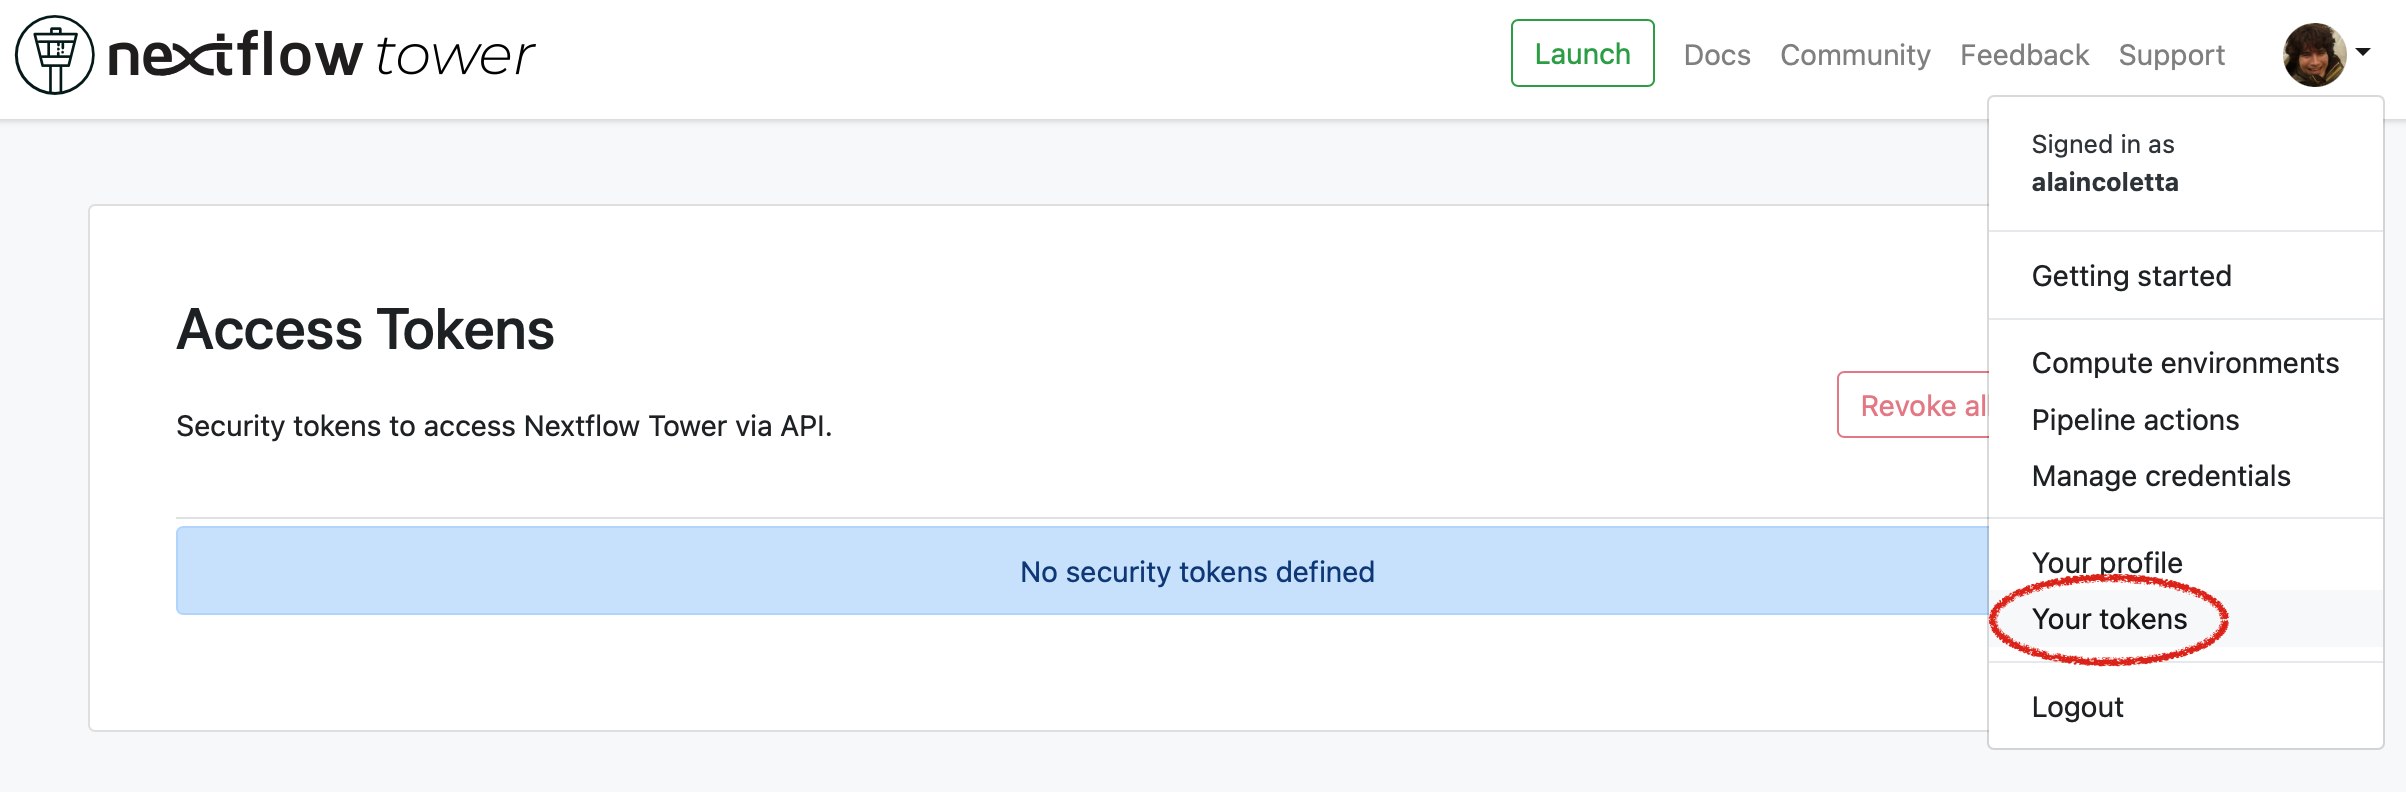
\includegraphics{img/usage_create_token.png}
\caption{Create a token}
\end{figure}

    \begin{enumerate}
\def\labelenumi{\arabic{enumi}.}
\setcounter{enumi}{2}
\tightlist
\item
  Name your token, this can be anything you like.
\end{enumerate}

    \begin{figure}
\centering
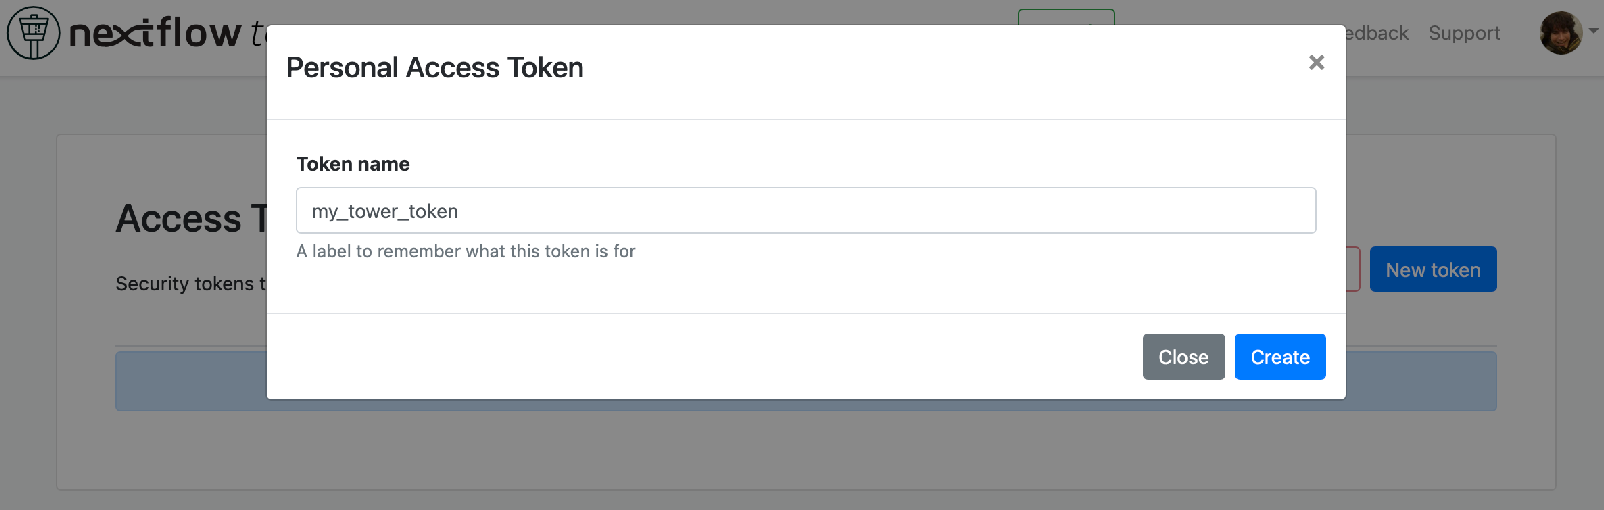
\includegraphics{img/name2.png}
\caption{Name the token}
\end{figure}

    \begin{enumerate}
\def\labelenumi{\arabic{enumi}.}
\setcounter{enumi}{3}
\tightlist
\item
  Copy your new token into a text editor and put in a safe place.
\end{enumerate}

    \begin{figure}
\centering
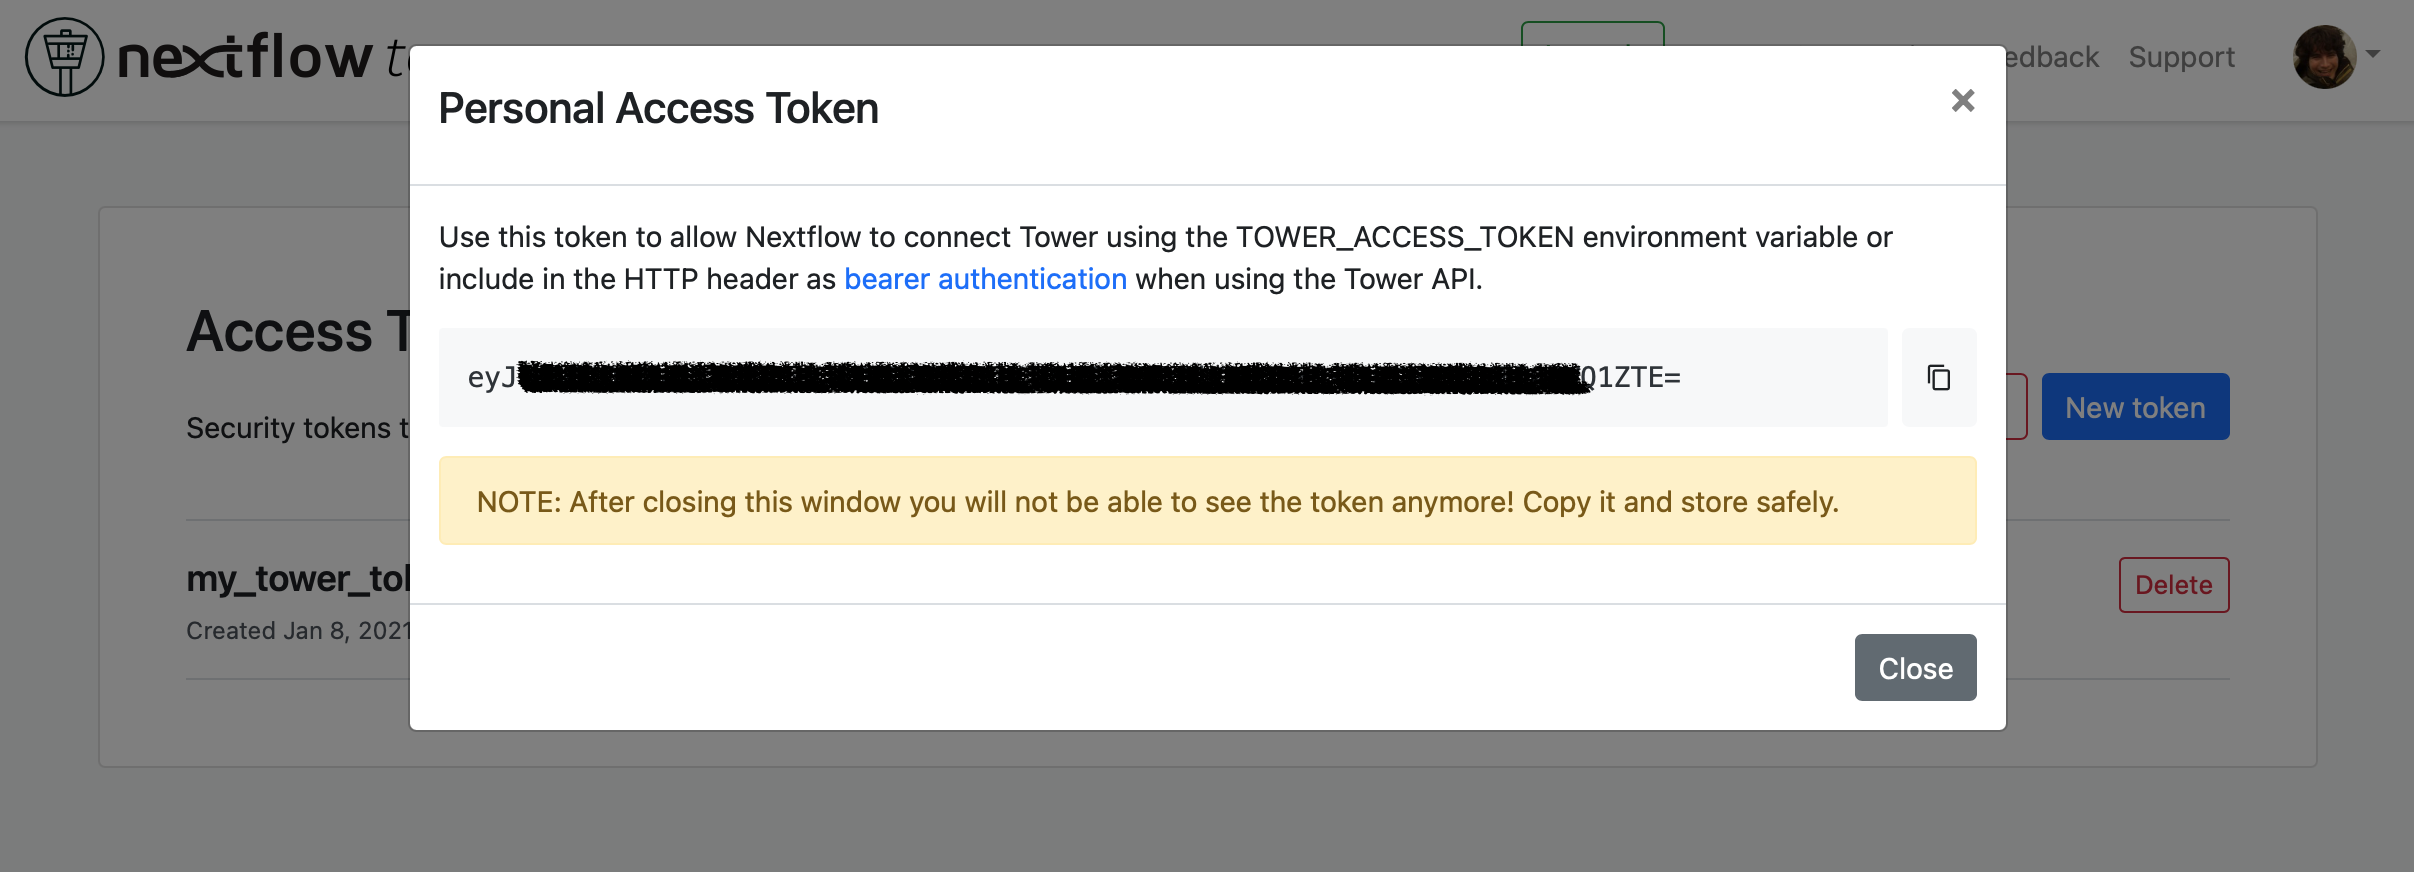
\includegraphics{img/usage_token.png}
\caption{Save the token}
\end{figure}

    \begin{enumerate}
\def\labelenumi{\arabic{enumi}.}
\setcounter{enumi}{4}
\tightlist
\item
  Once your token has been created, open a terminal and type:
\end{enumerate}

    \begin{tcolorbox}[breakable, size=fbox, boxrule=1pt, pad at break*=1mm,colback=cellbackground, colframe=cellborder]
\prompt{In}{incolor}{ }{\boxspacing}
\begin{Verbatim}[commandchars=\\\{\}]
\PY{n+nb}{export}\PY{+w}{ }\PY{n+nv}{TOWER\PYZus{}ACCESS\PYZus{}TOKEN}\PY{o}{=}eyxxxxxxxxxxxxxxxQ1ZTE
\end{Verbatim}
\end{tcolorbox}

    Where eyxxxxxxxxxxxxxxxQ1ZTE= is the token you have just created.

    Just a note to say that if you want this TOWER\_ACCESS\_TOKEN to be set
permanently then you can edit a file called \texttt{.bashrc} in your
home directory and add the above line to the end of the file.

    \hypertarget{installing-nextflow-pipelines}{%
\subsection{Installing Nextflow
Pipelines}\label{installing-nextflow-pipelines}}

The \texttt{nf-core/bactmap} pipeline is a bioinformatics best-practice
analysis pipeline for mapping short reads from bacterial WGS to a
reference sequence, creating filtered VCF files, making pseudogenomes
based on high quality positions in the VCF files and optionally creating
a phylogeny from an alignment of the pseudogenomes.

    \begin{figure}
\centering
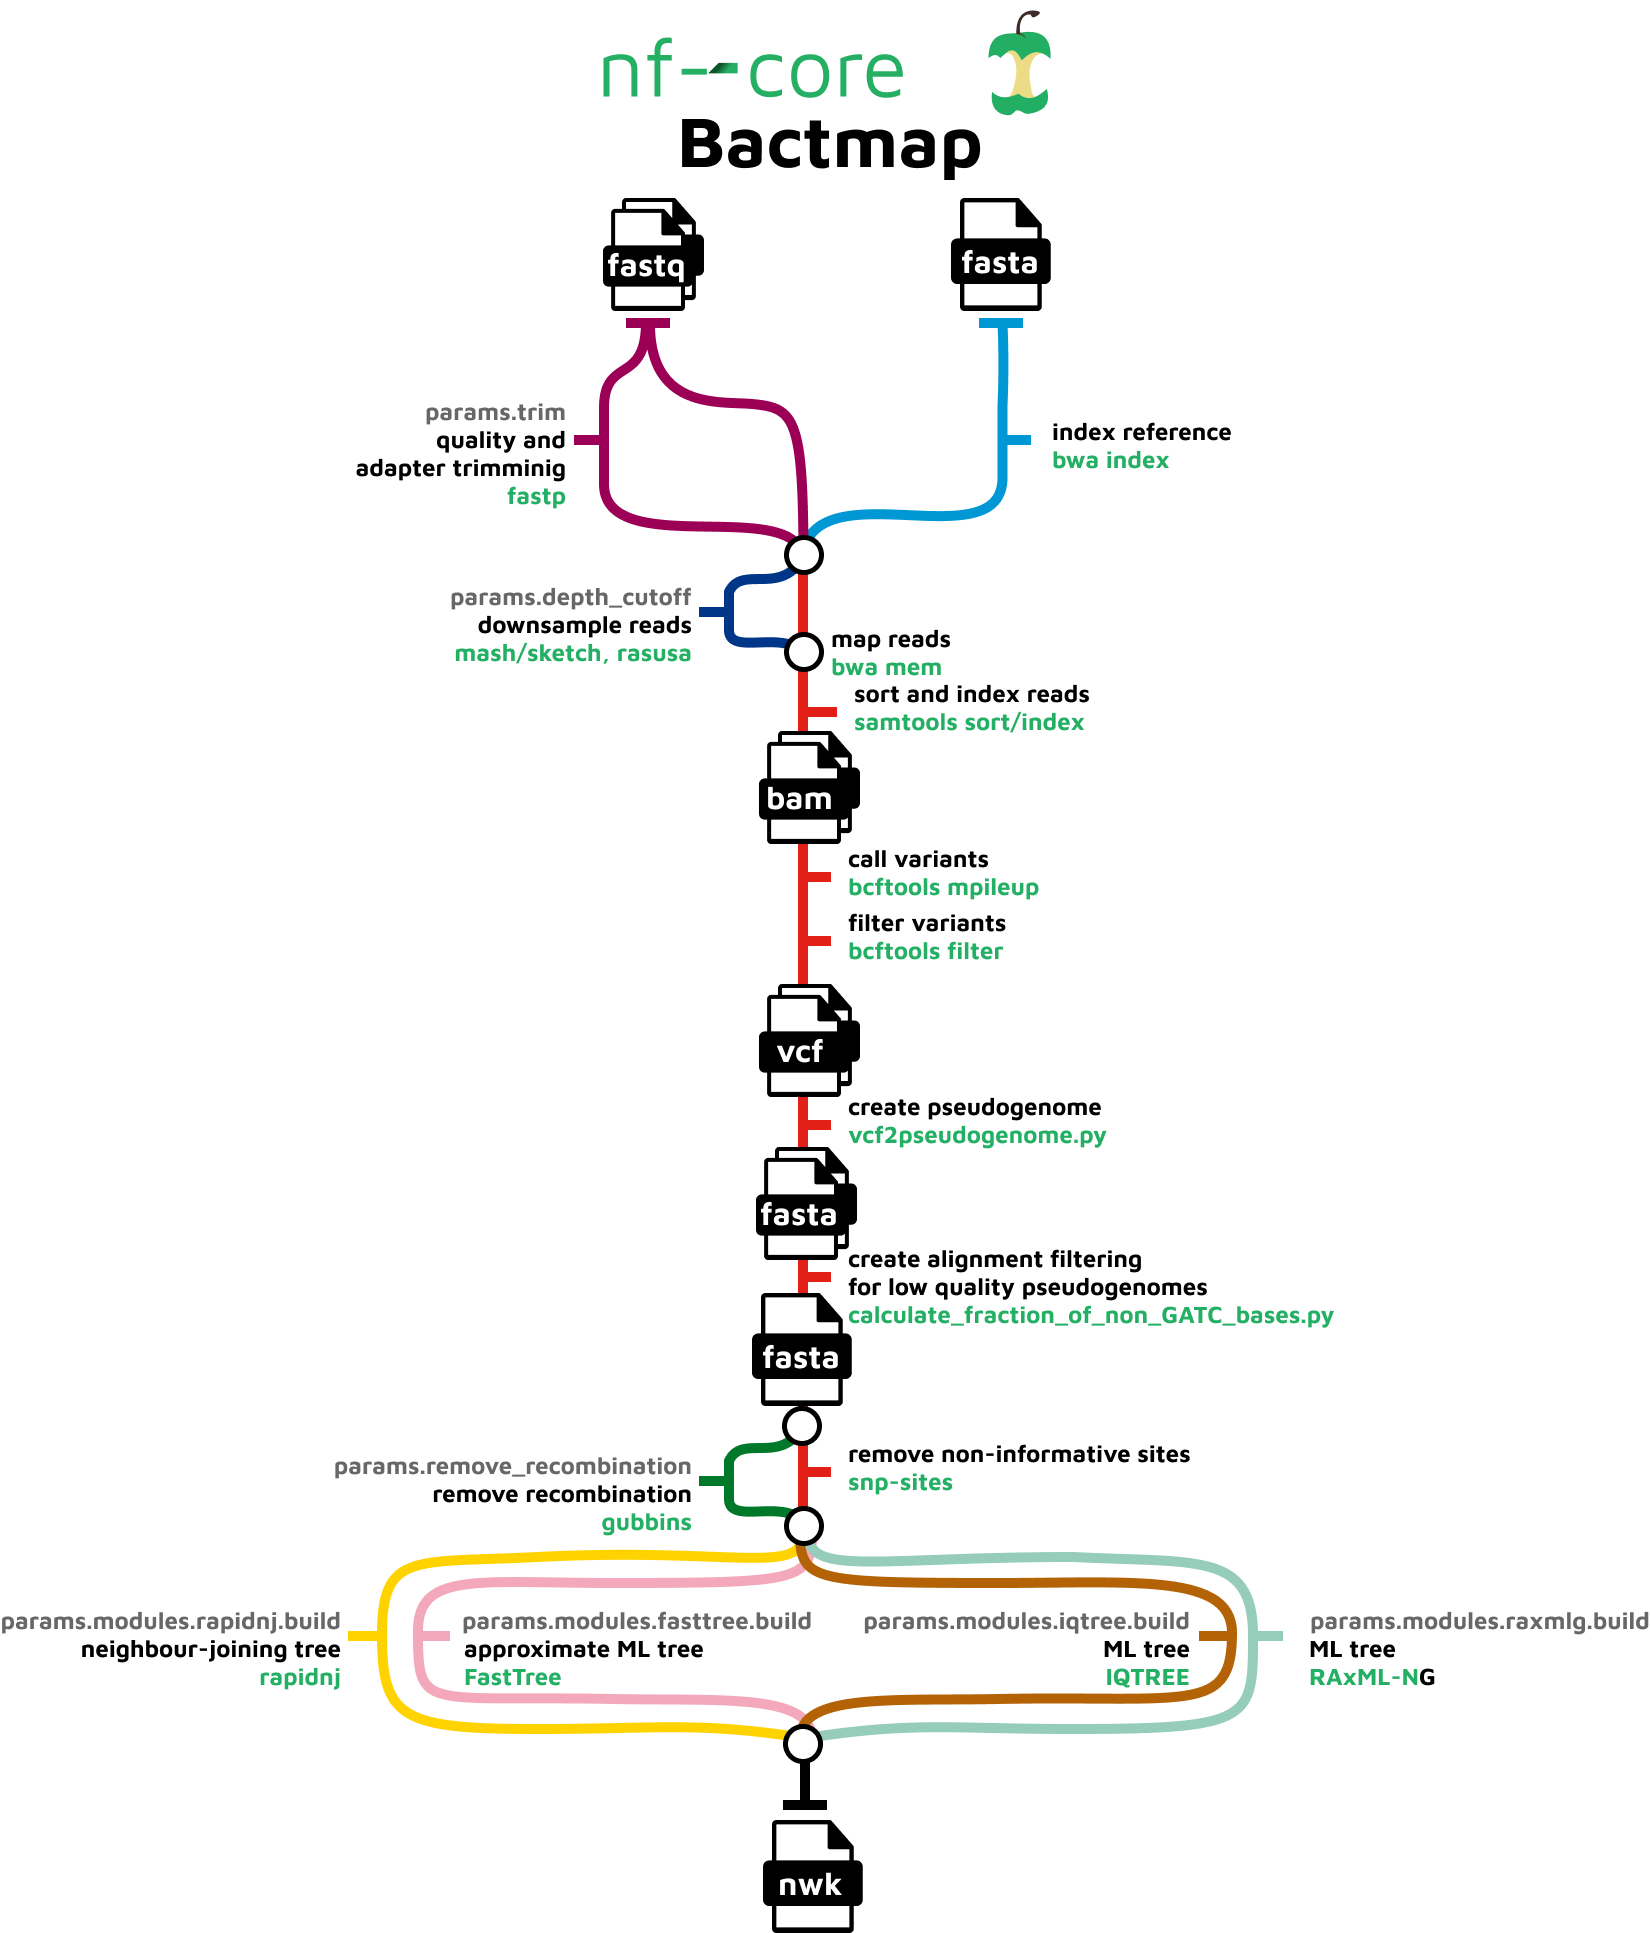
\includegraphics{img/Bactmap_pipeline.png}
\caption{Bactmap Pipeline Summary}
\end{figure}

    Before we install any nf-core pipelines we must first set up a directory
to hold the singularity containers for the software applications that
used in the pipelines.

    \begin{tcolorbox}[breakable, size=fbox, boxrule=1pt, pad at break*=1mm,colback=cellbackground, colframe=cellborder]
\prompt{In}{incolor}{ }{\boxspacing}
\begin{Verbatim}[commandchars=\\\{\}]
mkdir\PY{+w}{ }\PYZti{}/singularity
\PY{n+nb}{export}\PY{+w}{ }\PY{n+nv}{NXF\PYZus{}SINGULARITY\PYZus{}CACHEDIR}\PY{o}{=}\PY{l+s+s2}{\PYZdq{}\PYZti{}/singularity\PYZdq{}}
\end{Verbatim}
\end{tcolorbox}

    To install this \texttt{nf-core/bactmap} pipeline, type

    \begin{tcolorbox}[breakable, size=fbox, boxrule=1pt, pad at break*=1mm,colback=cellbackground, colframe=cellborder]
\prompt{In}{incolor}{ }{\boxspacing}
\begin{Verbatim}[commandchars=\\\{\}]
nf\PYZhy{}core\PY{+w}{ }download\PY{+w}{ }\PYZhy{}\PYZhy{}compress\PY{+w}{ }none\PY{+w}{ }\PYZhy{}\PYZhy{}container\PYZhy{}system\PY{+w}{ }singularity\PY{+w}{ }\PY{l+s+se}{\PYZbs{}\PYZbs{}}
\PYZhy{}\PYZhy{}revision\PY{+w}{ }\PY{l+m}{1}.0.0\PY{+w}{ }bactmap
\end{Verbatim}
\end{tcolorbox}

    This may take some time to install. This command will download the
nf-core pipeline called \texttt{bactmap}, the options
\texttt{-\/-compress\ none} indicate how to compress the output,
\texttt{-\/-container\ singularity} specifies to download singularity
container images for the required software and
\texttt{-\/-revision\ 1.0.0} specifies which version of bactmap to
install.

    Check that the pipeline has installed:

    \begin{tcolorbox}[breakable, size=fbox, boxrule=1pt, pad at break*=1mm,colback=cellbackground, colframe=cellborder]
\prompt{In}{incolor}{ }{\boxspacing}
\begin{Verbatim}[commandchars=\\\{\}]
ls\PY{+w}{ }nf\PYZhy{}core\PYZhy{}bactmap\PYZus{}1.0.0/1\PYZus{}0\PYZus{}0/
\end{Verbatim}
\end{tcolorbox}

    \hypertarget{running-nextflow-pipelines}{%
\subsection{Running Nextflow
Pipelines}\label{running-nextflow-pipelines}}

    Now that we have installed our first nextflow pipeline, let's run it on
some data. First we need to consult the pipeline documentation to see
how to run it. This can be found at
\url{https://nf-co.re/bactmap/1.0.0/docs/usage/}. In summary, we need to
create a samplesheet file with information about the samples in our
experiment. This file has to be a comma-separated file with 3 columns,
and a header row as shown in the example below.

    \texttt{sample,fastq\_1,fastq\_2}~\\
\texttt{G18582004,fastqs/G18582004\_1.fastq.gz,fastqs/G18582004\_2.fastq.gz}~\\
\texttt{G18756254,fastqs/G18756254\_1.fastq.gz,fastqs/G18756254\_2.fastq.gz}~\\
\texttt{G18582006,fastqs/G18582006\_1.fastq.gz,fastqs/G18582006\_2.fastq.gz}

    We have already created a samplesheet file for the data from the SNP
Phylogeny tutorial

    \begin{tcolorbox}[breakable, size=fbox, boxrule=1pt, pad at break*=1mm,colback=cellbackground, colframe=cellborder]
\prompt{In}{incolor}{ }{\boxspacing}
\begin{Verbatim}[commandchars=\\\{\}]
cat\PY{+w}{ }samplesheet.csv
\end{Verbatim}
\end{tcolorbox}

    Now run the \texttt{nf-core/bactmap} pipeline with

    \begin{tcolorbox}[breakable, size=fbox, boxrule=1pt, pad at break*=1mm,colback=cellbackground, colframe=cellborder]
\prompt{In}{incolor}{ }{\boxspacing}
\begin{Verbatim}[commandchars=\\\{\}]
nextflow\PY{+w}{ }run\PY{+w}{ }nf\PYZhy{}core\PYZhy{}bactmap\PYZus{}1.0.0/1\PYZus{}0\PYZus{}0/main.nf\PY{+w}{ }\PY{l+s+se}{\PYZbs{}}
\PYZhy{}\PYZhy{}input\PY{+w}{ }samplesheet.csv\PY{+w}{ }\PY{l+s+se}{\PYZbs{}}
\PYZhy{}\PYZhy{}outdir\PY{+w}{ }my\PYZus{}results\PY{+w}{ }\PY{l+s+se}{\PYZbs{}}
\PYZhy{}\PYZhy{}reference\PY{+w}{ }chromosome.fasta\PY{+w}{ }\PY{l+s+se}{\PYZbs{}}
\PYZhy{}\PYZhy{}iqtree\PY{+w}{ }\PY{l+s+se}{\PYZbs{}}
\PYZhy{}w\PY{+w}{ }my\PYZus{}results/work\PY{+w}{ }\PY{l+s+se}{\PYZbs{}}
\PYZhy{}profile\PY{+w}{ }singularity\PY{+w}{ }\PY{l+s+se}{\PYZbs{}}
\PYZhy{}resume\PY{+w}{ }\PY{l+s+se}{\PYZbs{}}
\PYZhy{}with\PYZhy{}tower
\end{Verbatim}
\end{tcolorbox}

    The pipeline steps that are to be run are written in the nextflow
language and are found in the file
\texttt{nf-core-bactmap\_1.0.0/1\_0\_0/main.nf}. Let's look at the
options, these can be seperated into two types.

The first set of options (starting with \texttt{-\/-}) are specific to
the \texttt{nf-core/bactmap} pipeline: * \texttt{-\/-input} specifies
the samplesheet.csv file that contains the fastq file information for
our samples\\
* \texttt{-\/-output} specifies the output where the results from the
pipeline will be saved\\
* \texttt{-\/-reference} specifies a fasta file of the reference
sequence\\
* \texttt{-\/-iqtree} specifies to build a tree using the IQ-TREE

The full set of parameters for the bactmap pipeline can be found at
\url{https://nf-co.re/bactmap/1.0.0/parameters/}.

The second set of options (starting with \texttt{-}) are specific to the
nextflow engine: * \texttt{-w} option tells nextflow where to store the
intermediate files produced by the pipeline\\
* \texttt{-profile} option tells nextflow to use the singularity
profile\\
* \texttt{-resume} option tells nextflow to run the script using the
cached results\\
* \texttt{-with-tower} option tells nextflow to send information about
the pipeline run to Nextflow Tower using the TOWER\_ACCESS\_TOKEN set
earlier

    \hypertarget{nextflow-profiles}{%
\subsubsection{Nextflow profiles}\label{nextflow-profiles}}

A profile is a set of configuration attributes that can be
activated/chosen when running a pipeline. One use of a profile is to
define a set of attributes specific to where you are running the
pipeline e.g.~singularity here tells Nextflow to run the pipeline
locally using Singularity containers.

There are a range of pre-configured profiles to use with nf-core
pipelines. If you were running the pipeline on a commercial cloud
platform (e.g.~google or amazon) you could use the specific profile for
that platform (e.g.~google or aws). If you were running the pipeline on
a compute cluster at your institute (e.g.~Sanger or Cambridge
University) you could use an institute specific profile provided someone
has implemented one in nf-core (e.g.~sanger or cambridge). A list of
available institute profiles can be found at
\url{https://github.com/nf-core/configs/}

    \hypertarget{nextflow-resume}{%
\subsubsection{Nextflow resume}\label{nextflow-resume}}

A very useful feature of Nextflow is the \texttt{-\/-resume} option that
can be used to re-start a pipeline if it fails. This will cache any
steps of the pipeline that run succesfully. When you fix the problem
with your data and re-run the pipeline it will not run all of the steps
from the beginning but instead it will start from the last failed step.

    \hypertarget{nextflow-tower}{%
\subsubsection{Nextflow tower}\label{nextflow-tower}}

You should be able to monitor your Nextflow jobs in Nextflow Tower. So
go back to the Nextflow Tower website and see if you can find your
pipeline run on the website. Nextflow Tower is extremely powerful, if
you have time explore the interface for your pipeline run. Notice it
lists all the steps of a pipeline run, the commands involved in each
step and tracks the compute resources (cpu time and memory) for the
pipeline.

    \begin{figure}
\centering
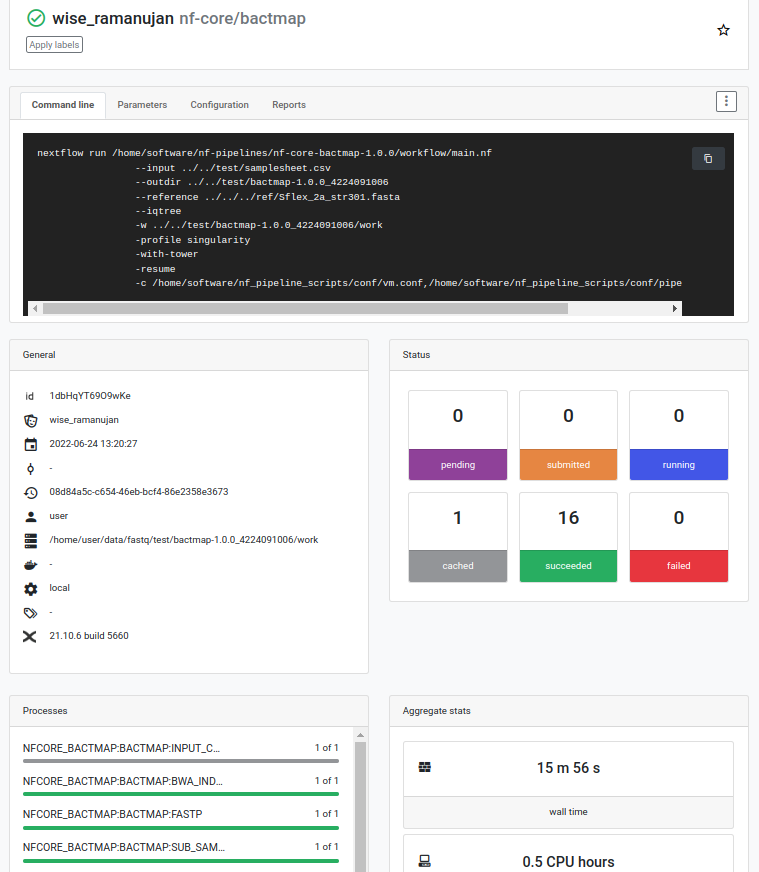
\includegraphics{img/tower.png}
\caption{Nextflow Tower}
\end{figure}

    \hypertarget{nextflow-tips}{%
\subsection{Nextflow Tips}\label{nextflow-tips}}

\begin{itemize}
\tightlist
\item
  Always take note of where you launced a nextflow pipeline from,
  pipeline progress will be stored in a hidden file called
  \texttt{.nextflow} in that directory
\item
  If running more than one nextflow pipeline at a time make sure to
  launch or start them from different directories
\item
  Remember to delete the work directory if the pipeline was successful
\end{itemize}

    Congratulations you have just successfully installed and run a nextflow
pipeline!


    % Add a bibliography block to the postdoc



\end{document}
